\pdfoutput=1
\documentclass[preview]{standalone}

\usepackage[utf8]{inputenc}
\usepackage{lmodern}
\usepackage[T1]{fontenc}

\usepackage{verbatim}
\usepackage{graphicx}
	\DeclareGraphicsRule{*}{mps}{*}{}
\usepackage{xcolor}

\usepackage{tikz}
	\usetikzlibrary{calc}
	\usetikzlibrary{arrows}
	\usetikzlibrary{backgrounds}
	\usetikzlibrary{decorations.pathmorphing}
	\usetikzlibrary{shapes.geometric}
	\tikzset{>=latex'}

\usepackage{amsmath}
\usepackage{amssymb}
\usepackage{dsfont}
\usepackage{nicefrac}
\usepackage{mathrsfs}
\usepackage[Euler]{upgreek}
\usepackage[nointegrals]{wasysym}
\usepackage{booktabs}
\usepackage{float}

\begin{document}

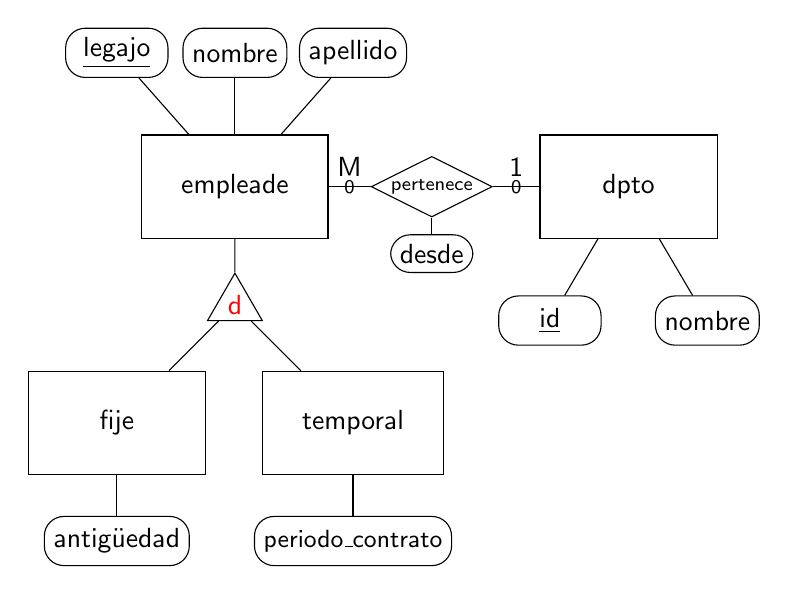
\begin{tikzpicture}[font=\sffamily]
	\node[draw,minimum width=2.25cm,inner sep=5mm] (empleade) at (0,0) {empleade};
	\node[draw,minimum width=2.25cm,inner sep=5mm] (dpto) at (5,0) {dpto};
	\node[draw,shape aspect=2,diamond,inner sep=0.2mm] (pertenece) at (2.5,0) {\scriptsize pertenece};
	\draw (empleade) -- node[above]{M} node{\scriptsize 0} (pertenece) -- node[above]{1} node{\scriptsize 0} (dpto);
	\node[draw,rounded corners=2.5mm,minimum width=1.3cm,minimum height=6.25mm] (legajo) at (-1.5,1.7) {$\underline{\text{legajo}}$};
	\node[draw,rounded corners=2.5mm,minimum width=1.3cm,minimum height=6.25mm] (nombre) at (0,1.7) {nombre};
	\node[draw,rounded corners=2.5mm,minimum width=1.3cm,minimum height=6.25mm] (apellido) at (1.5,1.7) {apellido};
	\draw (empleade)--(legajo);
	\draw (empleade)--(nombre);
	\draw (empleade)--(apellido);
	\node[draw,rounded corners=2.5mm,minimum width=1.3cm,minimum height=6.25mm] (id) at (4,-1.7) {$\underline{\text{id}}$};
	\node[draw,rounded corners=2.5mm,minimum width=1.3cm,minimum height=6.25mm] (nombre mat) at (6,-1.7) {nombre};
	\draw (dpto)--(id);
	\draw (dpto)--(nombre mat);
	\node[draw,rounded corners=2.5mm] (desde) at (2.5, -0.85) {desde};
	\draw (pertenece)--(desde);
	\node[draw,regular polygon,regular polygon sides=3,inner sep=0.2mm] (herencia) at (0,-1.5) {\textcolor{red}{d}};
	\node[draw,minimum width=2.25cm,inner sep=5mm] (fije) at (-1.5,-3.0) {fije};
	\node[draw,rounded corners=2.5mm,minimum width=1.3cm,minimum height=6.25mm] (attr1) at (-1.5,-4.5) {antigüedad};
	\node[draw,minimum width=2.25cm,inner sep=5mm] (temporal) at (1.5,-3.0) {temporal};
	\node[draw,rounded corners=2.5mm,minimum width=1.3cm,minimum height=6.25mm] (attr2) at (1.5,-4.5) {\small periodo\_contrato};
	\draw (fije)--(attr1) (temporal)--(attr2);
	\draw (empleade)--(herencia)--(fije) (herencia)--(temporal);
\end{tikzpicture}

\end{document}
